\section{Auswertung}
\label{sec:Auswertung}

% Schwellenstrom
\subsection{Bestimmen des Schwellenstroms}
Die in REF EINFÜGEN!!!\ref{sec:} beschriebene Lasergranulation tritt ab einem Strom von rund $I=\qty{34}{\milli\ampere}$ auf. Unterhalb dieses Grenzwertes ist das Licht
nicht monochromatisch und die Lasergranulation ist, wie in \autoref{fig:lasergranulation_1} zu sehen, nicht zu beobachten. Wird der Grenzwert eingestellt, ist zu beobachten,
dass die Intensität des Lichts stark zunimmt, was in \autoref{fig:lasergranulation_2} gezeigt wird.

  \begin{figure}
    \begin{subfigure}[c]{0.5\textwidth}
        \centering
        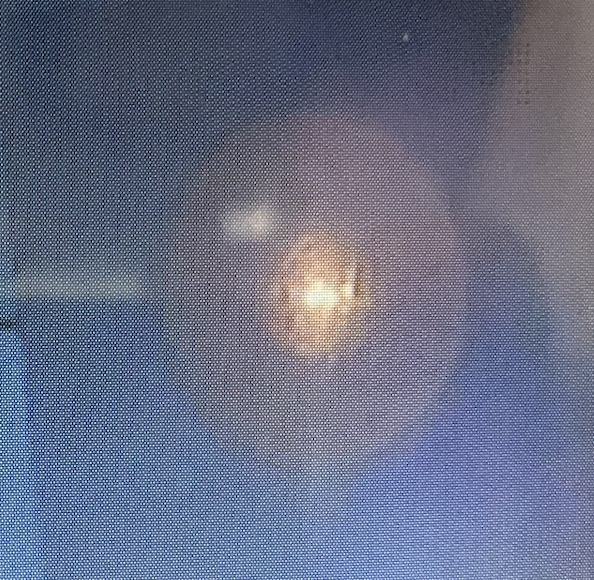
\includegraphics[width=0.6\textwidth]{content/pics/30mA.png}
        \subcaption{$I=\qty{30}{\milli\ampere}$}
    
    \end{subfigure}
    \begin{subfigure}[c]{0.5\textwidth}
        \centering
        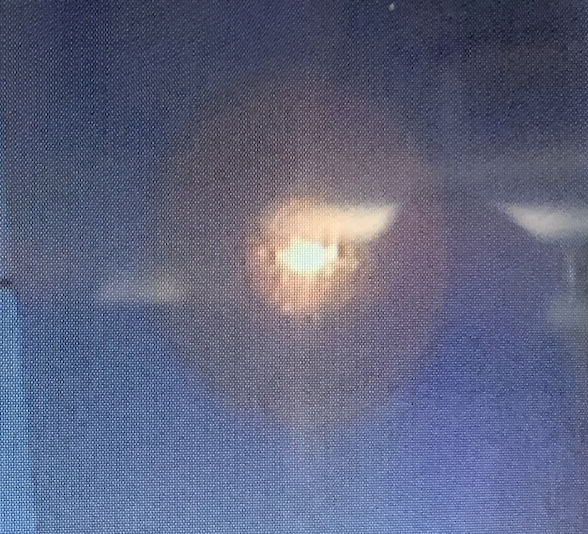
\includegraphics[width=0.6\textwidth]{content/pics/33,5mA.png}
        \subcaption{$I=\qty{33,5}{\milli\ampere}$}
    \end{subfigure}
    \caption{Bild des reflektierten Lichts für einen Ströme unterhalt des festgestellten Schwellenstroms. Die Lasergranulation ist nicht zu beobachten.}
    \label{fig:lasergranulation_1}
\end{figure}

\begin{figure}
    \begin{subfigure}[c]{0.5\textwidth}
        \centering
        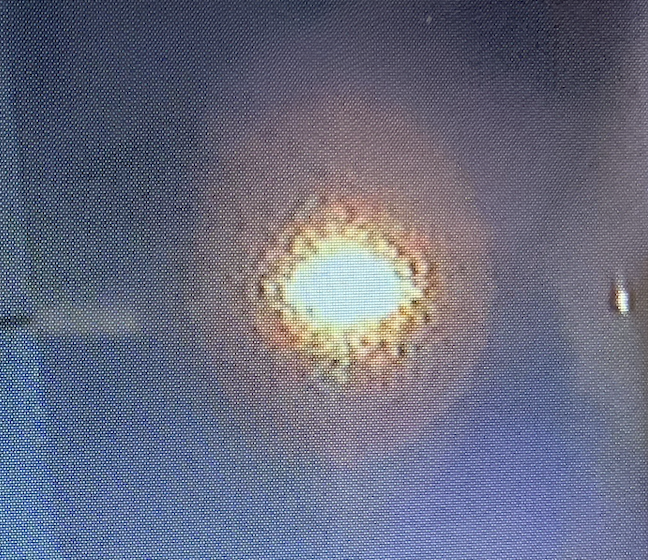
\includegraphics[width=0.6\textwidth]{content/pics/34mA.png}
        \subcaption{$I=\qty{34}{\milli\ampere}$}
    
    \end{subfigure}
    \begin{subfigure}[c]{0.5\textwidth}
        \centering
        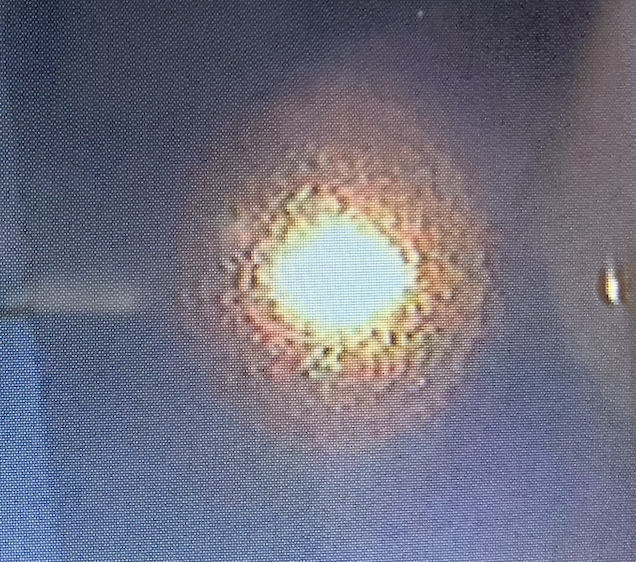
\includegraphics[width=0.6\textwidth]{content/pics/35mA.png}
        \subcaption{$I=\qty{35}{\milli\ampere}$}
    \end{subfigure}
    \caption{Bild der Lasergranulation für Ströme überhalb des festgestellten Schwellenstroms.}
    \label{fig:lasergranulation_2}
\end{figure}


% Rubidiumfluoreszenz
\subsection{Rubidiumfluoreszenz}
Die Rubidiumfluoreszenz wird für verschiedene Ströme beobachtet, eine Foto davon ist in \autoref{fig:Rubidiumfluoreszenz} zu sehen.

\begin{figure}
    \centering
    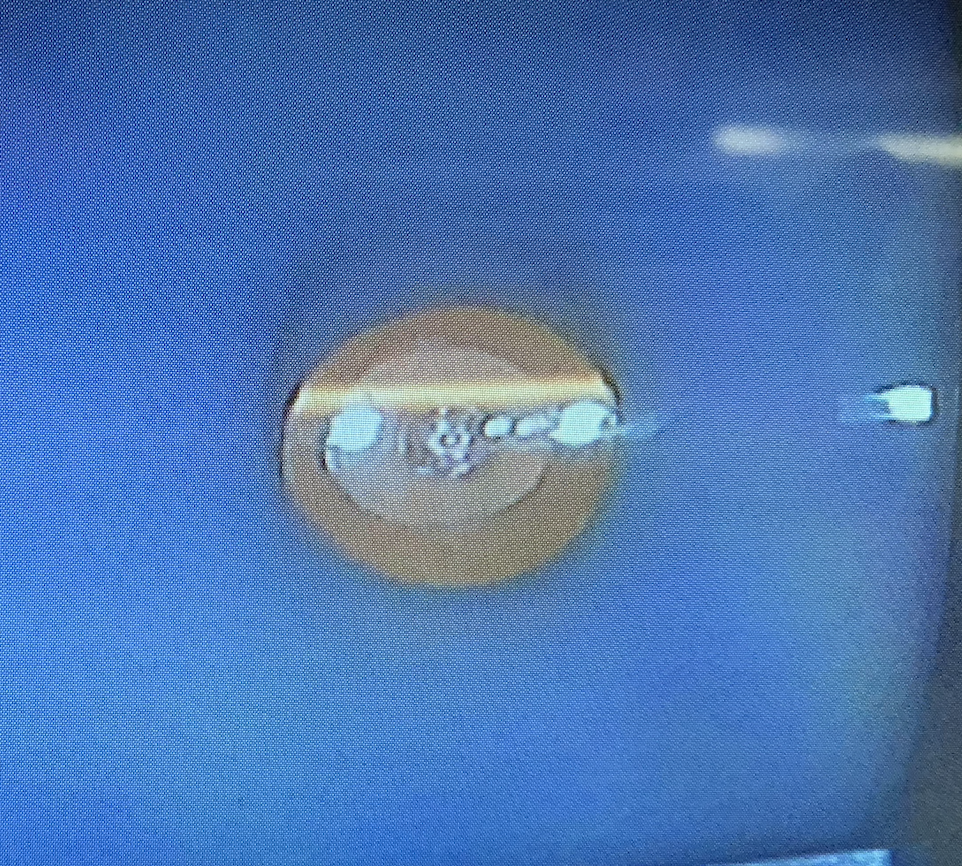
\includegraphics{content/pics/Fluoreszenz.png}
    \caption{Bild der zu beobachtenden Rubidiumfluoreszenz.}
    \label{fig:Rubidiumfluoreszenz}
\end{figure}

% Transmissionspektrum der Rubidiumzelle
\subsection{Transmissionsspektrum der Rubidiumzelle}
In \autoref{fig:Transmissionspektrum} ist das gemessene Transmissionspektrum der Rubidiumzelle aufgetragen. Aufgrund der Lage und Intensität der Peaks
lassen sich diese zu den in \autoref{fig:Rubidiumübergänge} FIG DAZU IN THEORIE????????? beschriebenenen Rubidiumübergängen zuordnen.

\begin{figure}
    \centering
    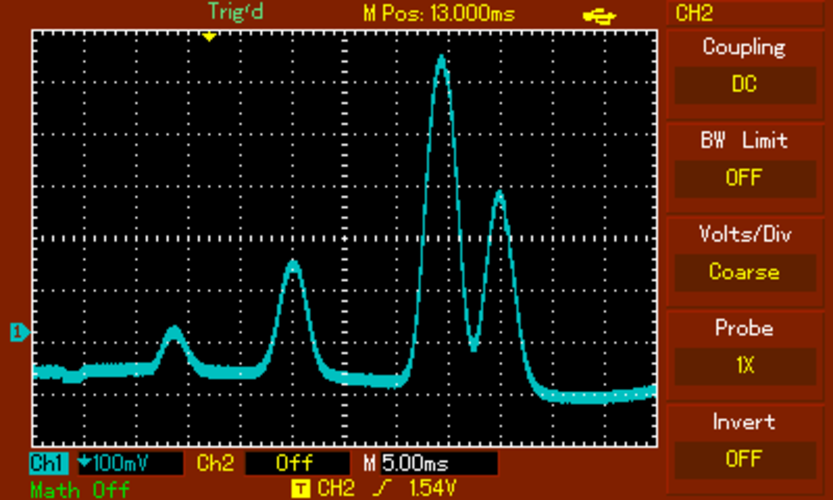
\includegraphics{content/pics/Peaks.pdf}
    \caption{Bild des Oszilloskopbildschirms. Zu sehen ist das Transmissionspektrum der Rubidiumzelle.}
    \label{fig:Rubidiumübergänge}
\end{figure}